%<dscrpt>Fichier de déclarations Latex à inclure au début d'un élément de cours.</dscrpt>

\documentclass[a4paper]{article}
\usepackage[hmargin={1.8cm,1.8cm},vmargin={2.4cm,2.4cm},headheight=13.1pt]{geometry}

%includeheadfoot,scale=1.1,centering,hoffset=-0.5cm,
\usepackage[pdftex]{graphicx,color}
\usepackage[french]{babel}
%\selectlanguage{french}
\addto\captionsfrench{
  \def\contentsname{Plan}
}
\usepackage{fancyhdr}
\usepackage{floatflt}
\usepackage{amsmath}
\usepackage{amssymb}
\usepackage{amsthm}
\usepackage{stmaryrd}
%\usepackage{ucs}
\usepackage[utf8]{inputenc}
%\usepackage[latin1]{inputenc}
\usepackage[T1]{fontenc}


\usepackage{titletoc}
%\contentsmargin{2.55em}
\dottedcontents{section}[2.5em]{}{1.8em}{1pc}
\dottedcontents{subsection}[3.5em]{}{1.2em}{1pc}
\dottedcontents{subsubsection}[5em]{}{1em}{1pc}

\usepackage[pdftex,colorlinks={true},urlcolor={blue},pdfauthor={remy Nicolai},bookmarks={true}]{hyperref}
\usepackage{makeidx}

\usepackage{multicol}
\usepackage{multirow}
\usepackage{wrapfig}
\usepackage{array}
\usepackage{subfig}


%\usepackage{tikz}
%\usetikzlibrary{calc, shapes, backgrounds}
%pour la présentation du pseudo-code
% !!!!!!!!!!!!!!      le package n'est pas présent sur le serveur sous fedora 16 !!!!!!!!!!!!!!!!!!!!!!!!
%\usepackage[french,ruled,vlined]{algorithm2e}

%pr{\'e}sentation du compteur de niveau 2 dans les listes
\makeatletter
\renewcommand{\labelenumii}{\theenumii.}
\renewcommand{\thesection}{\Roman{section}.}
\renewcommand{\thesubsection}{\arabic{subsection}.}
\renewcommand{\thesubsubsection}{\arabic{subsubsection}.}
\makeatother


%dimension des pages, en-t{\^e}te et bas de page
%\pdfpagewidth=20cm
%\pdfpageheight=14cm
%   \setlength{\oddsidemargin}{-2cm}
%   \setlength{\voffset}{-1.5cm}
%   \setlength{\textheight}{12cm}
%   \setlength{\textwidth}{25.2cm}
   \columnsep=1cm
   \columnseprule=0.5pt

%En tete et pied de page
\pagestyle{fancy}
\lhead{MPSI-\'Eléments de cours}
\rhead{\today}
%\rhead{25/11/05}
\lfoot{\tiny{Cette création est mise à disposition selon le Contrat\\ Paternité-Pas d'utilisations commerciale-Partage des Conditions Initiales à l'Identique 2.0 France\\ disponible en ligne http://creativecommons.org/licenses/by-nc-sa/2.0/fr/
} }
\rfoot{\tiny{Rémy Nicolai \jobname}}


\newcommand{\baseurl}{http://back.maquisdoc.net/data/cours\_nicolair/}
\newcommand{\urlexo}{http://back.maquisdoc.net/data/exos_nicolair/}
\newcommand{\urlcours}{https://maquisdoc-math.fra1.digitaloceanspaces.com/}

\newcommand{\N}{\mathbb{N}}
\newcommand{\Z}{\mathbb{Z}}
\newcommand{\C}{\mathbb{C}}
\newcommand{\R}{\mathbb{R}}
\newcommand{\D}{\mathbb{D}}
\newcommand{\K}{\mathbf{K}}
\newcommand{\Q}{\mathbb{Q}}
\newcommand{\F}{\mathbf{F}}
\newcommand{\U}{\mathbb{U}}
\newcommand{\p}{\mathbb{P}}


\newcommand{\card}{\mathop{\mathrm{Card}}}
\newcommand{\Id}{\mathop{\mathrm{Id}}}
\newcommand{\Ker}{\mathop{\mathrm{Ker}}}
\newcommand{\Vect}{\mathop{\mathrm{Vect}}}
\newcommand{\cotg}{\mathop{\mathrm{cotan}}}
\newcommand{\sh}{\mathop{\mathrm{sh}}}
\newcommand{\ch}{\mathop{\mathrm{ch}}}
\newcommand{\argsh}{\mathop{\mathrm{argsh}}}
\newcommand{\argch}{\mathop{\mathrm{argch}}}
\newcommand{\tr}{\mathop{\mathrm{tr}}}
\newcommand{\rg}{\mathop{\mathrm{rg}}}
\newcommand{\rang}{\mathop{\mathrm{rg}}}
\newcommand{\Mat}{\mathop{\mathrm{Mat}}}
\newcommand{\MatB}[2]{\mathop{\mathrm{Mat}}_{\mathcal{#1}}\left( #2\right) }
\newcommand{\MatBB}[3]{\mathop{\mathrm{Mat}}_{\mathcal{#1} \mathcal{#2}}\left( #3\right) }
\renewcommand{\Re}{\mathop{\mathrm{Re}}}
\renewcommand{\Im}{\mathop{\mathrm{Im}}}
\renewcommand{\th}{\mathop{\mathrm{th}}}
\newcommand{\repere}{$(O,\overrightarrow{i},\overrightarrow{j},\overrightarrow{k})$}
\newcommand{\cov}{\mathop{\mathrm{Cov}}}

\newcommand{\absolue}[1]{\left| #1 \right|}
\newcommand{\fonc}[5]{#1 : \begin{cases}#2 \rightarrow #3 \\ #4 \mapsto #5 \end{cases}}
\newcommand{\depar}[2]{\dfrac{\partial #1}{\partial #2}}
\newcommand{\norme}[1]{\left\| #1 \right\|}
\newcommand{\se}{\geq}
\newcommand{\ie}{\leq}
\newcommand{\trans}{\mathstrut^t\!}
\newcommand{\val}{\mathop{\mathrm{val}}}
\newcommand{\grad}{\mathop{\overrightarrow{\mathrm{grad}}}}

\newtheorem*{thm}{Théorème}
\newtheorem{thmn}{Théorème}
\newtheorem*{prop}{Proposition}
\newtheorem{propn}{Proposition}
\newtheorem*{pa}{Présentation axiomatique}
\newtheorem*{propdef}{Proposition - Définition}
\newtheorem*{lem}{Lemme}
\newtheorem{lemn}{Lemme}

\theoremstyle{definition}
\newtheorem*{defi}{Définition}
\newtheorem*{nota}{Notation}
\newtheorem*{exple}{Exemple}
\newtheorem*{exples}{Exemples}


\newenvironment{demo}{\renewcommand{\proofname}{Preuve}\begin{proof}}{\end{proof}}
%\renewcommand{\proofname}{Preuve} doit etre après le begin{document} pour fonctionner

\theoremstyle{remark}
\newtheorem*{rem}{Remarque}
\newtheorem*{rems}{Remarques}

\renewcommand{\indexspace}{}
\renewenvironment{theindex}
  {\section*{Index} %\addcontentsline{toc}{section}{\protect\numberline{0.}{Index}}
   \begin{multicols}{2}
    \begin{itemize}}
  {\end{itemize} \end{multicols}}


%pour annuler les commandes beamer
\renewenvironment{frame}{}{}
\newcommand{\frametitle}[1]{}
\newcommand{\framesubtitle}[1]{}

\newcommand{\debutcours}[2]{
  \chead{#1}
  \begin{center}
     \begin{huge}\textbf{#1}\end{huge}
     \begin{Large}\begin{center}Rédaction incomplète. Version #2\end{center}\end{Large}
  \end{center}
  %\section*{Plan et Index}
  %\begin{frame}  commande beamer
  \tableofcontents
  %\end{frame}   commande beamer
  \printindex
}


\makeindex
\begin{document}
\noindent

\debutcours{Fonctions d'une variable réelle : étude locale}{beta 2.2 \tiny{ le \today} }

L'étude des fonctions d'une variable réelle est répartie entre \href{\baseurl C2063.pdf}{divers documents}.
\section{Limites}
\subsection{\'Etude locale : mais où ?}
Précisons la notion \og d'extrémités\fg~ d'un intervalle $I$. On convient que l'extrémité droite de $I$ est $\max(I)$ si $I$ admet un plus grand élément, $\sup(I)$ si $I$ est majoré mais n'admet pas de plus grand élément et $+\infty$ si $I$ n'est pas majoré. De même l'extrémité gauche est $\min(I)$ si $I$ admet un plus petit élément, $\inf(I)$ si $I$ est minoré mais n'admet pas de plus petit élément et $-\infty$ si $I$ n'est pas minorée. On note $\overline{I}$ l'intervalle $I$ auquel on adjoint ses extrémités. Ainsi
\[
\overline{\R} = \R \cup \left\lbrace  -\infty\right\rbrace \cup \left\lbrace  +\infty\right\rbrace, \hspace{0.5cm}
\overline{\left] a,b\right] } = \left[ a,b \right] , \hspace{0.5cm}
\overline{\left] -\infty ,b\right[} = \left] -\infty,b\right] \cup \left\lbrace  -\infty\right\rbrace
\]
Dans ce chapitre, on s'intéresse à ce qui se passe autour d'un $a \in \overline{I}$ pour une fonction $f$ définie dans un intervalle $I$. Il faut bien noter que $a$ n'est pas forcément un point de $I$ c'est à dire que la fonction $f$ n'est pas forcément \emph{définie} en $a$. En revanche,
\begin{itemize}
 \item si $a\in\R$, pour tout $\alpha > 0$, $I\cap \left[ a-\alpha, a+\alpha \right] \neq \emptyset$,
 \item si $a = +\infty$, pour tout $A\in \R$, $I\cap \left[ A ,+\infty \right[ \neq \emptyset$,
 \item si $a = -\infty$, pour tout $A\in \R$, $I\cap \left] -\infty, A \right] \neq \emptyset$
\end{itemize}
Autrement dit, il existe des points arbitrairement proches de $a$ en lesquels la fonction est définie.

Notion de propriété \og locale en $a$\fg.

\subsection{Définitions}
\index{question de cours!les 9 définitions d'une limite}
\begin{defi}
 Les neuf cas pour la définition d'une limite $f\xrightarrow{a} l$ sont présentés dans le tableau suivant
\renewcommand{\arraystretch}{1.5}
\begin{center}
\begin{tabular}{c|c|l}
$a$        & $l$ & définition de $f\xrightarrow{a} l$ \\ \hline
\multirow{3}*{réel}   & $\in \R$ & 
     $\forall \varepsilon> 0,\; \exists \alpha_\varepsilon > 0 \text{ tq } \forall t\in I :
     |t-a| \leq \alpha_\varepsilon \Rightarrow |f(t)-l| \leq \varepsilon$ \\ \cline{2-3}
           & $=-\infty$ &
     $\forall E\in \R,\; \exists \alpha_E >0 \text{ tq } \forall t\in I :
     |t-a| \leq \alpha_E \Rightarrow f(t) \leq  E $ \\ \cline{2-3}
           & $=+\infty$ &
$\forall E\in \R,\; \exists \alpha_E >0 \text{ tq } \forall t\in I :
|t-a| \leq \alpha_E \Rightarrow f(t)> E $ \\ \hline \hline
\multirow{3}*{$ -\infty$} & $\in \R$ &
$\forall \varepsilon> 0,\; \exists A_\varepsilon \in \R \text{ tq } \forall t\in I :
t \leq  A_\varepsilon \Rightarrow |f(t)-l| \leq \varepsilon$ \\ \cline{2-3}
           & $=-\infty$ &
$\forall E\in \R,\; \exists A_E \in \R \text{ tq } \forall t\in I :
t \leq  A_E \Rightarrow f(t) \leq E$ \\ \cline{2-3}
           & $=+\infty$ &
$\forall E\in \R,\; \exists A_E \in \R \text{ tq } \forall t\in I :
t \leq  A_E \Rightarrow f(t) > E$  \\ \hline \hline
\multirow{3}*{$+\infty$}  & $\in \R$ &
$\forall \varepsilon> 0,\; \exists A_\varepsilon \in \R \text{ tq } \forall t\in I :
t \geq A_\varepsilon \Rightarrow |f(t)-l| \leq \varepsilon$ \\ \cline{2-3}
           & $=-\infty$ &
$\forall E\in \R,\; \exists A_E \in \R \text{ tq } \forall t\in I :
t \geq A_\varepsilon \Rightarrow f(t) \leq E$ \\ \cline{2-3}
           & $=+\infty$ &
$\forall E\in \R,\; \exists A_E \in \R \text{ tq } \forall t\in I :
t \geq A_\varepsilon \Rightarrow f(t)>E$ 
\end{tabular}
\end{center}
\end{defi}
Notations usuelles pour les limites.
\begin{displaymath}
  \lim_{x\rightarrow a}f(x) = l,\hspace{1cm} \lim_{a}f = l,\hspace{1cm}
  f(x)\xrightarrow{x \rightarrow a}l, \hspace{1cm} f \xrightarrow{a}l 
\end{displaymath}
Les notations 2 et 4 sont à préférer car elles mettent mieux en avant que ce sont des \emph{fonctions} qui admettent des limites et non des nombres. On peut aussi utiliser la flèche de convergence  avec les conventions habituelles de notation des fonctions \emph{anonymes}:
\begin{displaymath}
\left(
\begin{aligned}
  \left]0,+\infty \right[ &\rightarrow \R \\ x&\mapsto \frac{1}{x} 
\end{aligned} 
\right) \xrightarrow{0} +\infty
\end{displaymath}

On introduit des notions de limites à droite ou à gauche, stricte ou large en un point $a$.\index{limite à droite, à gauche} Il s'agit des limites des \emph{restrictions} de la fonction aux intervalles
\begin{itemize}
 \item $I\cap \left] -\infty , a \right]$ pour une limite à gauche (large),
 \item $I\cap \left] -\infty , a \right[$ pour une limite à gauche stricte,
 \item $I\cap \left[ a, +\infty \right[$ pour une limite à droite (large),
 \item $I\cap \left] a, +\infty \right[$ pour une limite à gauche stricte.
\end{itemize}
Ces notions sont analogues aux suites extraites. Notations $f\xrightarrow{a+}l$ (droite), $f\xrightarrow{a++}l$ (droite stricte), $f\xrightarrow{a-}l$ (gauche), $f\xrightarrow{a--}l$ (gauche stricte). 
\begin{rems}
\begin{itemize}
 \item Si une fonction admet une limite $l$ en $a$ alors elle admet aussi $l$ pour limite en $a$ à gauche ou à droite stricte ou large.
 \item Attention  $\left( f\xrightarrow{a++}l \text{ et } f\xrightarrow{a--}l\right) $ n'entraine pas  $f\xrightarrow{a}l$.
\end{itemize}
\end{rems}
On peut étendre de la notion de limite en $a$ lorsque $f$ est définie dans $I\setminus\left\lbrace a\right\rbrace$. (pour la dérivabilité et les développements limités)
\begin{defi}
 Soit $I$ un intervalle, $a\in I$ et $f$ une fonction définie dans $I\setminus\left\lbrace a\right\rbrace$. On dit que $f$ admet $l$ pour limite en $a$ si et seulement si les resctictions à droite et à gauche de $a$ admettent $l$ pour limite en $a$. 
\end{defi}

\subsection{Propriétés}\index{passage à la limite dans une inégalité pour une fonction} \index{stabilité des inégalités larges par passage à la limite}
\index{fonction localement bornée}
\begin{defi}[fonction localement bornée]
  Une fonction $f$ définie dans un intervalle $I$ est localement bornée en $a\in I$ (ou au voisinage de $a$) si et seulement si il existe un $\alpha > 0$ tel que $f_{|I\cap[a-\alpha,a+\alpha]}$ soit bornée.
\end{defi}
On peut étendre la définition: $f$ est localement bornée au voisinage de $+\infty$ (respectivement $-\infty$) si et seulement si il existe $A\in \R$ tel que 
$f_{|[A,+\infty[}$ (respectivement $f_{|]-\infty, A]}$) soit bornée.
\begin{prop}
Une fonction qui converge en $a$ est localement bornée au voisinage de $a$. 
\end{prop}
\begin{demo}
 à compléter
\end{demo}

\begin{prop}
 Si $f$ converge en $a$ vers $l$ et si $l\neq 0$, il existe un voisinage de $a$ dans lequel $f$ est non nulle du signe de $l$ avec $|f|\geq \frac{|l|}{2}$. 
\end{prop}
\begin{demo}
 à compléter
\end{demo}

\begin{thm}[Passage à la limite dans une inégalité]
  Soit $I$ un intervalle et $a\in \overline{I}$. Soit $f$, $g$ deux fonctions définies dans $I$. Si $f \xrightarrow{a} l_f$, $g \xrightarrow{a} l_g$ et si $f \leq g$ au voisinage de (localement en ) $a$, alors $l_f \leq l_g$. 
\end{thm}
\begin{demo}
 à compléter
\end{demo}

Conséquence : Unicité de la limite \index{unicité de la limite}. 

\begin{thm}[Théorème d'encadrement.]
  Soit $I$ un intervalle et $a\in \overline{I}$. Soit $f$, $g$, $h$ trois fonctions définies dans $I$ telles que $f\leq g \leq h$ dans un voisinage de (localement en) $a$.
\[
\left. 
\begin{aligned}
 f &\xrightarrow{a} l \\ h &\xrightarrow{a} l
\end{aligned}
\right\rbrace \Rightarrow g \xrightarrow{a} l, \hspace{0.5cm}
f \xrightarrow{a} +\infty \Rightarrow g \xrightarrow{a} +\infty, \hspace{0.5cm}
h \xrightarrow{a} -\infty \Rightarrow g \xrightarrow{a} -\infty
\]
\end{thm}
\begin{demo}
 à compléter
\end{demo}


\subsection{Continuité}
\begin{rem}
 $a\in I$ et  $f\xrightarrow{a}l$ entraine $l=f(a)$.
\end{rem}
\begin{defi}[fonction continue en $a$]
  Soit $f$ définie dans $I$ et $a\in I$. On dit que $f$ est continue en $a$ si et seulement si $f\xrightarrow{a}f(a)$.
\end{defi}
\begin{defi}[fonction continue dans un intervalle]
 Soit $I$ un intervalle réel et $f$ une fonction définie dans $I$. On di que $f$ est \emph{continue dans $I$} si et seulement si , pour tout $a\in I$, la fonction $f$ est continue en $a$.
\end{defi}

\index{fonctions continues}

\section{Opérations}
Le plan est à peu près le même que pour l'étude des \href{\baseurl C2069.pdf}{suites convergentes}.
\begin{prop}
  Le produit d'une fonction localement bornée en $a$ par une fonction qui converge vers $0$ en $a$ converge vers $0$. Le produit de deux fonctions qui convergent vers $0$ en $a$ converge vers $0$ en $a$. La somme de deux fonctions qui convergent vers $0$ en $a$ converge vers $0$ en $a$.
\end{prop}
\begin{demo}
  à rédiger
\end{demo}

\begin{thm}[Opérations sur les fonctions convergentes]
 Soit  $I$ un intervalle de $\R$, $a\in\overline{I}$ et $f$, $g$ deux fonctions définies dans $I$ et qui convergent en $a$ respectivement vers des réels $l_f$ et $l_g$. Soit $\lambda$ un nombre réel. Les fonctions résultats des opérations présentées dans le tableau suivant convergent en $a$ vers les limites indiquées.
\begin{center}
\renewcommand{\arraystretch}{1.5}
\begin{tabular}{c|c|c|c|c|c|c|}
opérations  & $|f|$ & $f+g$ &  $\lambda f$ & $fg$ & $\sup(f,g)$ & $\inf(f,g)$\\ \hline
limites & $|l_f|$ & $\lambda l_f$ & $l_f+l_g$ & $l_fl_g$ & $\max(l_f,l_g)$ & $\min(l_f,l_g)$
\end{tabular}
\end{center}
\end{thm}
\begin{demo}
Les démonstrations se font en écrivant des inégalités exploitées par le théorème d'encadrement.
 \begin{description}
 \item[valeur absolue] La propriété repose sur l'inégalité
\begin{displaymath}
 \left\vert |f(x)| -|l_f|\right\vert \leq |f(x) - l_f|
\end{displaymath}
\item[somme] $\left| (f+g)(x) - (l_f+l_g)\right| \leq  \left| f(x) - l_f\right| + \left| g(x) - l_g \right|$.
\item[multiplication externe] $\left|\lambda f(x) - \lambda l_f\right| = |\lambda|\left|f(x) - l_f\right|$.
\item[produit] On introduit un terme croisé
\[
 \left| (fg)(x) - (l_fl_g)\right| \leq |g(x)| \left| f(x) - l_f\right| + |l_f|\left| g(x) - l_g \right|.
\]

\item[sup et inf] La propriété repose sur les propriétes déjà montrées ainsi que sur les formules :
\begin{align*}
 \sup(f,g) = \dfrac{1}{2}(f+g+|f-g|) & & \inf(f,g) = \dfrac{1}{2}(f+g - |f-g|)
\end{align*}
\end{description}
\end{demo}
On peut faire un tableau analogue à celui pour les suites relativement aux opérations sur les fonctions qui divergent vers $+\infty$ ou $-\infty$.
Dans les tableaux suivant sont rassemblées de \og bonnes\fg~ hypothèses relativement à des opérations comprenant des fonctions admettant des limites infinies.
\begin{center}
\renewcommand{\arraystretch}{1.3}
% use packages: array
\begin{tabular}{l|l|l}
Propriété de $f$ & Propriété de $g$ & Propriété de $f + g$\\ \hline
localement (en $a$) minorée & $\rightarrow+\infty$ & $\rightarrow+\infty$ \\ \hline
localement (en $a$) majorée & $\rightarrow-\infty$ & $\rightarrow-\infty$
\end{tabular}
\end{center}
\begin{center}
\renewcommand{\arraystretch}{1.3}
% use packages: array
\begin{tabular}{l|l|l}
Propriété de $f$ & Propriété de $g$ & Propriété de $fg$\\ \hline
localement (en $a$) minorée par un nombre $>0$. & $\rightarrow+\infty$ & $\rightarrow+\infty$ \\ \hline
localement (en $a$) majorée par un nombre $<0$ & $\rightarrow-\infty$ & $\rightarrow +\infty$\\ \hline
localement (en $a$) majorée par un nombre $<0$ & $\rightarrow+\infty$ & $\rightarrow -\infty$\\ \hline
localement (en $a$) minorée par un nombre $>0$ & $\rightarrow-\infty$ & $\rightarrow -\infty$\\ \hline
\end{tabular}
\end{center}
\begin{demo}
  à compléter
\end{demo}


\section{Composition}
\subsection{Caractérisation séquentielle de la continuité}
\index{caractérisation séquentielle de la continuité}
\begin{thm}[caractérisation séquentielle de la limite]
  Soit $a\in \overline{I}$, $l\in \overline{\R}$ et $f$ définie dans $I$. Alors $f$ admet $l$ pour limite en $a$ si et seulement si pour toute suite $\left( x_n\right)_{n\in \N}$ d'éléments de $I$ qui converge vers $a$, la suite $\left( f(x_n)\right)_{n\in \N} \rightarrow l$
\end{thm}
\index{question de cours!caractérisation séquentielle de la continuité}
\begin{demo}
  Suivant que $a$ et $l$ sont réels ou $+\infty$ ou $-\infty$, diverses démonstrations analogues sont à fournir. On se place dans le cas où $a$ et $l$ sont finis, les autres cas sont à rédiger.
  \begin{itemize}
    \item Convergence de la fonction entraîne convergence des suites. On suppose $f\rightarrow l$, on considère une suite $\left( x_n\right)_{n\in \N}$ quelconque qui converge vers $a$.
  Pour tout $\varepsilon >0$,\newline
  1 - Il existe un $\alpha_\varepsilon > 0$ tel que $|x-a|\leq \alpha_\varepsilon \Rightarrow |f(x)-l|\leq \varepsilon$ car $f\rightarrow l$.\newline
  2 - Pour ce $\alpha_\varepsilon > 0$, il existe un $N\in \N$ tel que $n\geq N \Rightarrow |x_n-a|\leq \alpha_\varepsilon$.\newline
  3 - Alors $n\geq N \Rightarrow |f(x_n)-l|\leq \varepsilon$.
    \item On doit montrer que si, pour \emph{toute} suite $\left( x_n\right)_{n\in \N}$ qui converge vers $a$, la suite $\left( f(x_n)\right)_{n\in \N}$ converge vers $l$, alors $f\rightarrow l$ en $a$. On va prouver la contraposée c'est à dire que si $f$ ne converge pas vers $l$ en $a$ alors il existe une suite $\left( x_n\right)_{n\in \N}$ qui converge vers $a$ mais pour laquelle la suite $\left( f(x_n)\right)_{n\in \N}$ ne converge pas vers $l$.\newline
    On suppose donc que $f$ ne converge pas vers $l$ en $a$.\newline
    Il existe\footnote{En général le nom $\varepsilon$ vient toujours après un quantificateur $\forall$, le $\exists$ vient ici de la négation de la proposition habituelle} donc un $\varepsilon$ particulier (notons le $\varepsilon_0$ tel que, pour tout $\alpha >0$ (en particulier pour $\frac{1}{n}$) il existe un $x$ (notons le $x_n$ car il dépend de $n$) tel que
\begin{displaymath}
  |x_n - a| \leq \frac{1}{n} \hspace{0.5cm}\text{ et } \hspace{0.5cm}|f(x_n)-l|\geq \varepsilon_0
\end{displaymath}
La première inégalité montre par le théorème d'encadrement que $\left( x_n\right)_{n\in \N}\rightarrow a$ et la deuxième que $\left( x_n\right)_{n\in \N}$ ne converge pas vers $l$ (le théorème de passage à la limite dans une inégalité entrainerait une contradiction).
  \end{itemize}
\end{demo}

\subsection{Composition de fonctions}
\begin{thm}
 Soit $I$ un intervalle et $a\in \overline{I}$. Soit $f$ une fonction définie dans $I$ qui admet une limite $l$ en $a$.\newline
 Soit $J$ un intervalle tel que $l\in \overline{J}$ et $f(I)\subset J$.\newline
 Soit $g$ une fonction définie dans $J$ qui admet une limite $\lambda$ en $l$.\newline
 La fonction $g\circ f$ admet alors la limite $\lambda$ en $a$.
\end{thm}
\begin{demo}
 Parmi les 27 cas possibles pour $a$, $l$, $\lambda$ réels ou non, choisissons en un seulement, les autres sont analogues.\newline
 Par exemple $a=-\infty$, $l\in \R$, $\lambda = + \infty$. On veut montrer que $g \circ f \xrightarrow{-\infty} +\infty$.\newline
 Pour tout $E\in \R$.
 \begin{enumerate}
  \item Comme $g \xrightarrow{l} +\infty$, il existe $\alpha > 0$ tel que, pour tout $y\in J$, $|y - l |\leq \alpha \Rightarrow g(y) \geq E$.
  \item Comme $f\xrightarrow{a} l$, $\forall \varepsilon > 0,\, \exists A_\varepsilon\in \R$ tel que, $x\leq A_\varepsilon \Rightarrow \left|f(x) - l \right| \leq \varepsilon$. On considère en particulier $\varepsilon = \alpha$ et le $A_\alpha$.
 \end{enumerate}
Pour tout $x\in I$, 
\[
x\leq A_\alpha \Rightarrow \left|f(x) - l \right| \leq \alpha 
\Rightarrow g(f(x)) \geq E \text{ car } f(x) \in J.
\]
\end{demo}


\section{Fonctions monotones}
\index{question de cours!limites d'une fonction monotone} \index{théorème de la limite monotone}
\begin{prop}
 Soit $f$ une fonction monotone définie dans un intervalle $I$ et $a$ un point de $I$ qui n'est pas une extrémité. Alors $f$ admet en $a$ des limites strictement à droite et à gauche de $a$ notées $f_+(a)$ et $f_-(a)$.
\renewcommand{\arraystretch}{1.5}
\begin{center}
\begin{tabular}{c | c || c}
&$f$ croissante                                                         &  $f$ décroissante\\ \hline 
$f_-(a)$&$f\xrightarrow{a--} \sup\left\lbrace f(t), t\in I, t<a \right\rbrace $ & $f\xrightarrow{a--} \inf\left\lbrace f(t), t\in I, t<a \right\rbrace $\\  \hline
$f_+(a)$&$f\xrightarrow{a++} \inf\left\lbrace f(t), t\in I, t>a \right\rbrace $ & $f\xrightarrow{a++} \sup\left\lbrace f(t), t\in I, t>a \right\rbrace $\\  \hline
\end{tabular}
\end{center}
De plus, $f_-(a)\leq f(a) \leq f_+(a)$ si $f$ est croissante et $f_+(a)\leq f(a) \leq f_-(a)$ si $f$ est décroissante. La fonction est continue en $a$ si et seulement si $f_-(a)= f(a) = f_+(a)$.
\end{prop}
\begin{demo}
Remarquons d'abord que les parties de $\R$ 
\[
 I\cap \left] -\infty , a \right[ ,\hspace{0.5cm} \left\lbrace f(x) \text{ tq } x\in I, x < a \right\rbrace, \hspace{0.5cm} 
  I\cap \left] a, +\infty \right[ ,\hspace{0.5cm} \left\lbrace f(x) \text{ tq } x\in I, a < x\right\rbrace
\]
sont non vides car $a$ n'est pas une extrémité de $I$.\newline
Plaçons nous dans le cas où la fonction $f$ est croissante. Alors
\begin{align*}
 \left( \forall x \in I, x < a \Rightarrow f(x) \leq f(a)\right) 
 &\Rightarrow f(a) \text{ majore } \left\lbrace f(x) \text{ tq } x\in I, x < a \right\rbrace
 &\Rightarrow \sup \left\lbrace f(x) \text{ tq } x\in I, x < a \right\rbrace \leq f(a) \\
 \left( \forall x \in I, a < x \Rightarrow f(a) \leq f(x)\right) 
 &\Rightarrow f(a) \text{ minore } \left\lbrace f(x) \text{ tq } x\in I, a < x\right\rbrace 
 &\Rightarrow f(a)\leq  \inf\left\lbrace f(x) \text{ tq } x\in I, a < x\right\rbrace.
\end{align*}
Notons $f_-(a) = \sup \left\lbrace f(x) \text{ tq } x\in I, x < a \right\rbrace$ et montrons que c'est la limite de $f$ strictement à droite de $a$.\newline
Pour tout $\varepsilon >0$, le réel $f_-(a) - \varepsilon$ n'est pas un majorant de $\left\lbrace f(x) \text{ tq } x\in I, x < a \right\rbrace$. Il existe donc $u_\varepsilon \in I$ tel que $u_\varepsilon < a$ et $f_-(a) - \varepsilon < f(u_\varepsilon) \leq f_-(a) = \sup \left\lbrace f(x) \text{ tq } x\in I, x < a \right\rbrace$. Comme $f$ est croissante,
\[
 \forall x \in I, u_\varepsilon \leq x < a \Rightarrow f_-(a) - \varepsilon < f(u_\varepsilon) \leq f(x) \leq f_-(a).
\]
On en déduit que $f_-(a)$ est la limte de $f$ strictement à gauche de $a$. La démonstration pour le limite strictement à droite est analogue en considérant $f_+(a) + \varepsilon$.

Dans le cas où la fonction $f$ est décroissante, on se ramène eau cas croissant en utilisant $-f$ et les opérations usuelles.
\end{demo}
\begin{rem}
 Dans le cas où $a$ est une extrémité de l'intervalle, on ne peut considérer qu'un seul côté de l'intervalle. La limite stricte de ce côté existe encore etson expression est la même. 
\end{rem}

\index{continuité d'une application croissante sur un intervalle}
\index{question de cours!continuité d'une application croissante sur un intervalle (démonstration)}
\begin{thm}[continuité d'une application croissante sur un intervalle]
 Soit $f$ une fonction monotone définie dans un intervalle $I$. Si $f(I)$ est un intervalle, alors, pour tout $a\in I$, la fonction $f$ est continue en $a$. La fonction est donc continue dans $I$.
\end{thm}
\begin{demo}
En fait, on va démontrer la contraposée. Soit $f$ une fonction monotone dans $I$. On la suppose croissante (on se ramène à ce cas en considérant $-f$). Soit $a\in I$ tel que $f$ ne soit pas continue en $I$.\newline
Si $a$ n'est pas l'extrémité gauche de $I$, la discontinuité se traduit par $f_-(a) < f(a)$. Montrons que les points de $\left] f_-(a),f(a)\right[$ ne sont pas des images par $f$.
En effet:
\[
 x < a \Rightarrow f(x) \leq f_-(a) \hspace{0.5cm}\text{ et }\hspace{0.5cm} a \leq x \Rightarrow f(a) \leq f(x).
\]
Ceci montre que \emph{$f(I)$ n'est pas convexe}, il n'est donc pas un intervalle.\newline
Si $f$ est monotone et $f(I)$ est un intervalle, la situation précédente ne peut se produire pour aucun $a\in I$. La fonction doit donc être continue en tous les $a\in I$.
\end{demo}

\section{Extension aux fonctions à valeurs complexes}
\subsection{Opérations}
\begin{defi}
  Soit $f$ définie dans un intervalle $I$ de $\R$ et $a\in \overline{I}$. Soit $z\in \C$. La fonction $f$ converge en $a$ vers $z$ (notation $f\xrightarrow{a} z$ si et seulement si $|f-z|\xrightarrow{a} 0$.
\end{defi}
\begin{rems}
  \begin{itemize}
    \item La convergence d'une fonction à valeurs complexes se ramène donc à celle d'une fonction à valeurs réelles.
    \item On peut considérer $a$ réel ou $+\infty$ ou $-\infty$ mais la limite $z$ doit être dans $\C$.
  \end{itemize}
\end{rems}
\begin{prop}
  Soit $I$ un intervalle, $a\in \overline{I}$, $f$ et $g$ définies dans $I$ qui convergent respectivement en $a$ vers $l_f$ et $l_g$, $\lambda \in \C$. Alors:
\begin{displaymath}
\overline{f} \xrightarrow{a} \overline{l_f}, \hspace{0.5cm} |f|\xrightarrow{a} |l_f|, \hspace{0.5cm} f+g \xrightarrow{a}l_f + l_g, \hspace{0.5cm}
\lambda f \xrightarrow{a} \lambda l_f, \hspace{0.5cm} fg \xrightarrow{a} l_f l_g, \hspace{.5cm} \text{ si } l_f\neq 0:\: \frac{1}{f}\xrightarrow{a} \frac{1}{l_f}
\end{displaymath}
\end{prop}
\begin{demo}
  La démonstration repose sur des inégalités de module liées à l'inégalité triangulaire.
\end{demo}
\begin{prop}
  Soit $I$ un intervalle, $a\in \overline{I}$, $f$ définie dans $I$. Soit $z\in \C$.
\begin{displaymath}
  f \xrightarrow{a} z \Leftrightarrow \left( \Re(f) \xrightarrow{a} \Re(z) \text{ et } \Im(f) \xrightarrow{a} \Im(z) \right) 
\end{displaymath}
\end{prop}
\begin{demo}
  Dans un sens, on utilise $|\Re(f) - \Re(z)| \leq |f-z|$ et $|\Im(f) - \Im(z)| \leq |f-z|$. Dans l'autre, on utilise les opérations (linéarité) de la proposition précédente. 
\end{demo}

\subsection{Interprétation comme courbe paramétrée et branches infinies}
Ce paragraphe n'est pas au programme de MPSI.

Remarques sur les définitions possibles de la notion de branches infinie\index{branche infinie}. On se limite à un cas particulier
\begin{displaymath}
 \Vert \overrightarrow{Af(t)}\Vert \xrightarrow[t_0]{} +\infty
\end{displaymath}
Cette propriété est indépendante du point $A$.
\begin{figure}[!ht]
 \centering
 \input{C6430_3.pdf_t}
 \caption{Direction asymptotique}
\end{figure}

\begin{defi}[branche infinie avec direction asymptotique]\index{direction asymptotique}
 On dira que $f$ admet en $t_0$ une branche infinie avec une direction asymptotique $\overrightarrow{u}$ lorsqu'il existe un point $A$ tel que :
\begin{displaymath}
 \Vert \overrightarrow{Af(t)}\Vert \xrightarrow[t_0]{} +\infty 
\text{ et }
 \dfrac{\overrightarrow{Af(t)}}{\Vert \overrightarrow{Af(t)}\Vert} \xrightarrow[t_0]{} \overrightarrow{u}
\end{displaymath}
\end{defi}
Vérifions que la convergence et la valeur de la limite sont indépendantes du point $A$.
\begin{figure}
 \begin{center}
  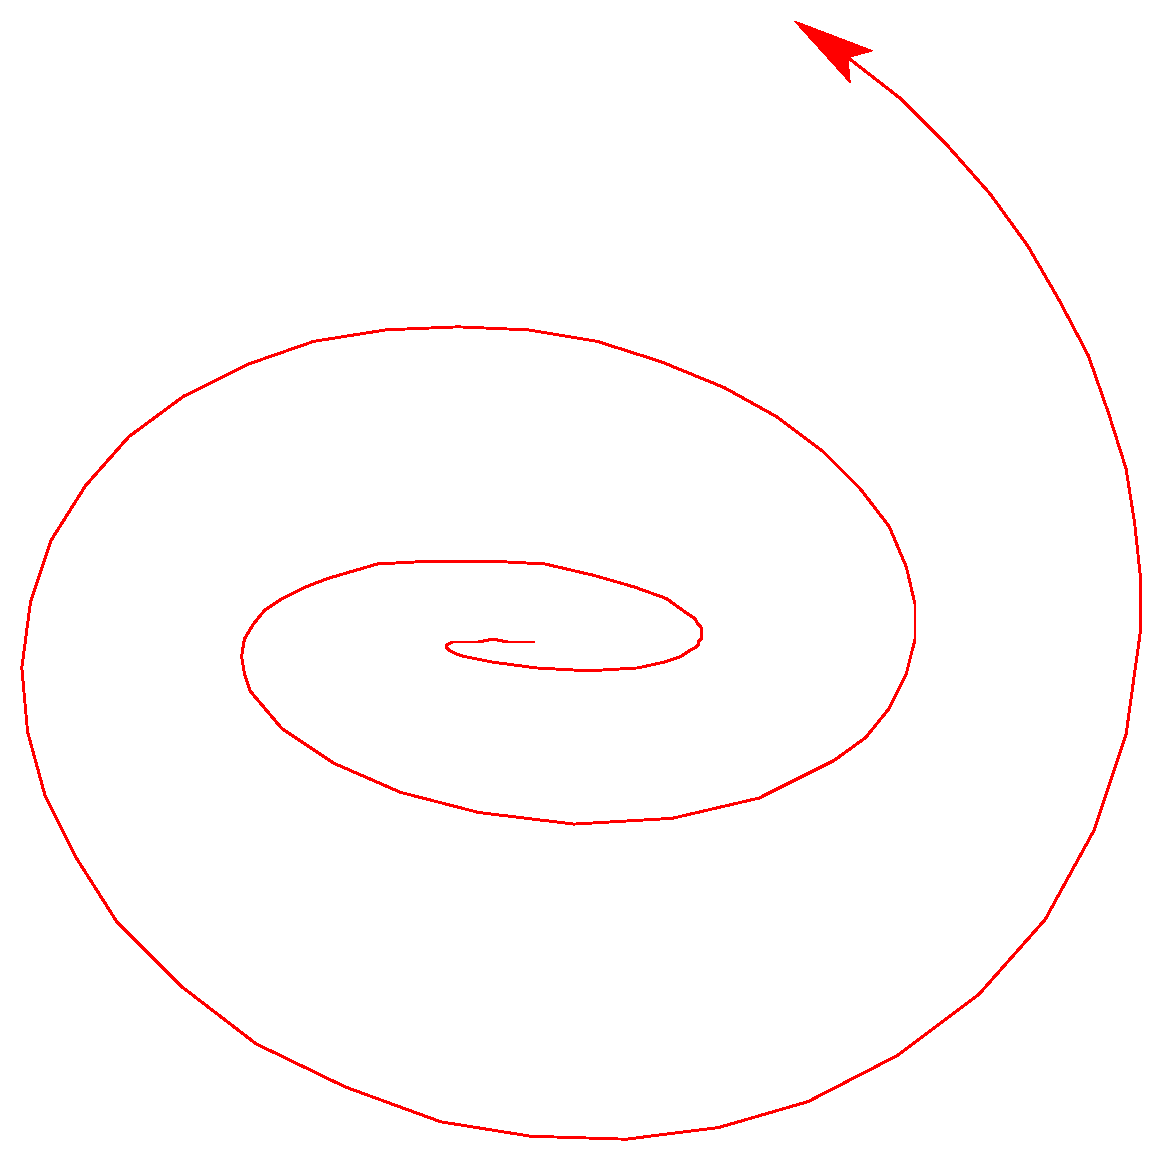
\includegraphics[width=6cm]{C6430_4.pdf}
 % C6430_3.pdf: 556x556 pixel, 72dpi, 19.61x19.61 cm, bb=0 0 556 556
\end{center}
\caption{branche infinie sans direction asymptotique}
\end{figure}

\begin{defi}[Asymptote]\index{asymptote}
 On dira que $f$ admet une branche infinie avec une droite asymptote $\mathcal D$ lorsque 
\begin{displaymath}
 \Vert \overrightarrow{Af(t)}\Vert \xrightarrow[t_0]{} +\infty 
\text{ et }
d(f(t),\mathcal D) \xrightarrow[t_0]{} 0
\end{displaymath}
\end{defi}
\begin{prop}
 Une courbe paramétrée $f$ admet une branche infinie avec une droite asymptote si et seulement si elle admet une directions asymptotique $\overrightarrow u$ et qu'il existe un point $A$ et un réel $l_A$ tel que
\begin{displaymath}
 \det(\overrightarrow{Af(t)},\overrightarrow u)\xrightarrow[t_0]{} l_A
\end{displaymath}
Dans ce cas, la droite asymptote est formée par les points $M$ tels que
\begin{displaymath}
 \det(\overrightarrow{Af(t)},\overrightarrow u)= l_A
\end{displaymath}
\end{prop}
\begin{demo}
  Vérifions que si on change de point, on change de limite $l_A$ mais pas de droite.
  Montrons que la distance de $f(t)$ à cette droite tends vers $0$.
\end{demo}
La proposition précédente conduit à une équation de l'asymptote et constitue une méthode pratique.\index{sf branches infinies}
\begin{exples}
\begin{enumerate}
 \item Courbes paramétrées $f(t)=O+u(t)\overrightarrow i +v(t)\overrightarrow j$ avec $u$ ou $v$ qui tend vers l'infini.à rédiger
 \item Cas d'une courbe en polaire : 
\begin{displaymath}
\left. 
\begin{aligned}
 f(\theta)=O+\rho(\theta)\overrightarrow{e}_{\theta}\\
\rho \xrightarrow[\theta_0]{} +\infty
\end{aligned}
\right\rbrace 
\Rightarrow \frac{1}{\Vert\overrightarrow{Of(\theta)} \Vert}\overrightarrow{Of(\theta)} = \overrightarrow{e}_{\theta} 
\xrightarrow[\theta_0]{} \overrightarrow{e}_{\theta_O}
\end{displaymath}
Il y a donc toujours une direction asymptotique. Il y a une asymptote si et seulement si le déterminant converge or
\begin{displaymath}
 \det(\overrightarrow{Of(\theta)},\overrightarrow{e}_{\theta_O}) = \rho(\theta)\sin(\theta - \theta_0)
\end{displaymath}
On obtient donc une forme indéterminée que l'on traite avec les outils de l'analyse. Lorsqu'il existe une limite finie $l$, on obtient une équation polaire de la droite asymptote qu'il est facile d'exprimer en coordonnées cartésiennes en développant simplement le $\sin$.
\begin{displaymath}
 \rho \sin(\theta -\theta_0) = l
\Leftrightarrow
-x\sin\theta_0 + y\cos\theta_0 = l
\end{displaymath}
\end{enumerate}
\end{exples}

\end{document}
